\section{Korrelationsgrafer}
\label{DatabehandlingKorrelationsgrafer}
%
Som beskrevet udføres der en PCA analyse relativt til forskellige grupperinger. Ud fra disse PCA analyser ses det, at nogle af de fundme og testede parametre korrlerer. For yderliger at undersøge disse korrelationer opsættes relevante grafer, hvor forholdet mellem de forskellige parametre og skala spørgsmål visualiseres. På alle grafer i det følgende afsnit vil x-aksen indikere testpersoner, men ikke nødvendigvis i kronologisk rækkefølge, hvorfor værdier på x-aksen er fjernet.

\subsubsection{Korrelation relativt til højde}
Når PCA analysen udføres relativt til højde, tyder det, som beskrevet i \fullref{DatabehandlingRHeight}, på, at en positiv korrelation mellem følgende parametre finder sted:
\begin{itemize}
	\item SQ12 og SQ18
	\item SQ14 og SQ15
	\item SQ8 og SQ17
\end{itemize}
%
Derudover ses der negativ korrelation mellem følgende parametre:
\begin{itemize}
	\item SQ12 og S21
	\item SQ18 og SQ21
	\item SQ2 og SQ9
	\item SQ4 og SQ9
	\item SQ16 og SQ19
\end{itemize}
%
På \autoref{fig:SammenligningSQ12SQ18} ses sammenhængen mellem SQ12 og SQ18, hvor der kan se en tendens i at når testpersonerne kan lide at blive betjent af robotten synes de også at robotten er spændende. 
%
\begin{figure}[H]
	\centering
	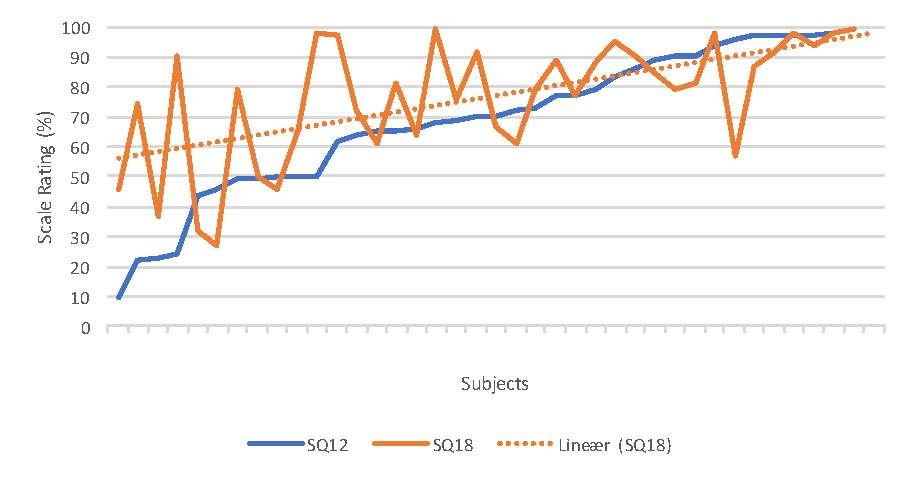
\includegraphics[width=\textwidth]{Figure/Korrelationsgrafer/SQ12+SQ18}
	\caption{Sammenhæng mellem hvad testpersonerne angiver (\%) på skalaen til SQ12: \textit{Jeg kan godt lide at blive betjent af robotten} og SQ18: \textit{Hvad synes du om robotten?}. At den orange kurve ikke er kontinuerlig skyldes, at nogle testpersoner ikke har angivet en respons på skalaen.}
	\label{fig:SammenligningSQ12SQ18}
\end{figure}
\noindent
%
På \autoref{fig:SammenligningSQ14SQ15} ses sammenhængen mellem SQ14 og SQ15. Kigges der på tendenslinjen kan der tilnærmelsesvis ses en sammenhæng mellem de to parametre, men kigges der på punkterne på grafen virker det ikke umiddelbart til at hvor personlig robottens hjælp blev oplevet og hvor overrasket testpersonerne blev over henvendelsen har indflydelse på hinanden.
%
\begin{figure}[H]
	\centering
	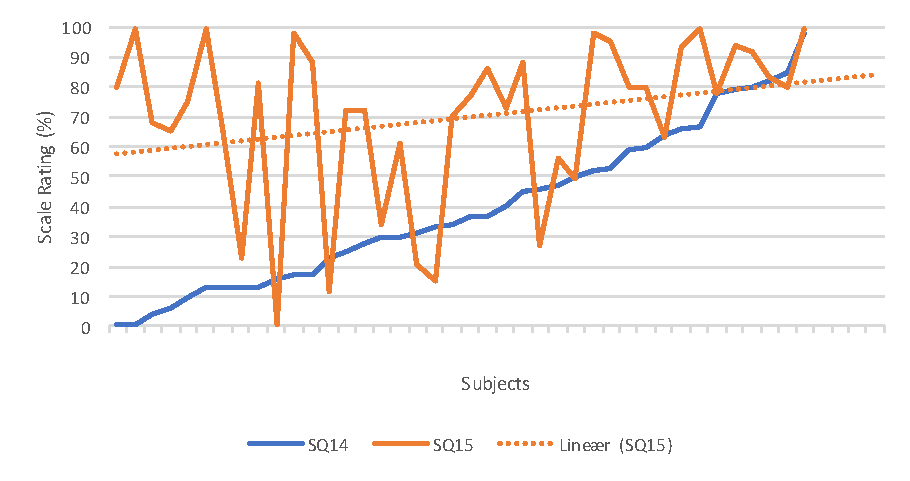
\includegraphics[width=\textwidth]{Figure/Korrelationsgrafer/SQ14+SQ15}
	\caption{Sammenhæng mellem hvad testpersonerne angiver (\%) på skalaen til SQ14: \textit{Hvor personlig oplevede du robottens hjælp?} og SQ15: \textit{Hvor overrasket blev du over robottens henvendelse?}.}
	\label{fig:SammenligningSQ14SQ15}
\end{figure}
\noindent
%
På \autoref{fig:SammenligningSQ8SQ17} ses der en lille tendens, hvor robotten rates mere elegant, når testpersonerne føler robotten kan hjælpe dem. Igen ligger datapunkterne dog meget spredt, så det betyder ikke nødvendigvis at en direkte sammenhæng er tilfældet. 
%
\begin{figure}[H]
	\centering
	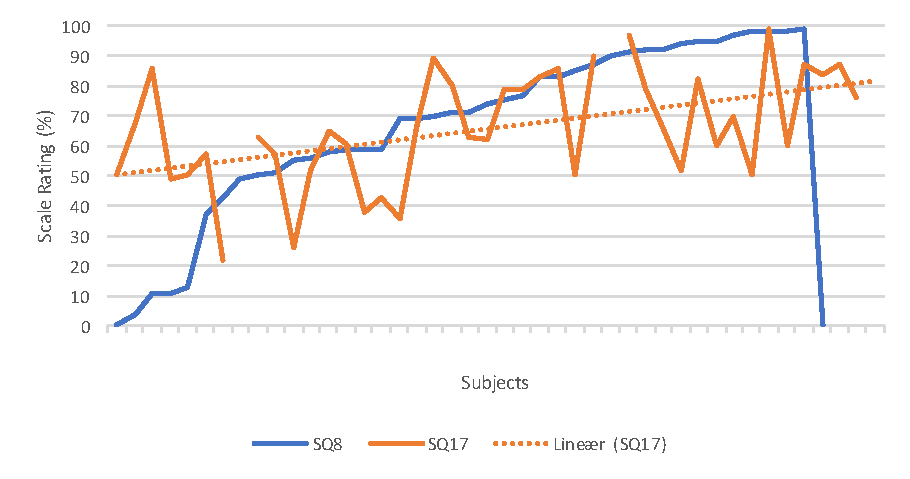
\includegraphics[width=\textwidth]{Figure/Korrelationsgrafer/SQ8+SQ17}
	\caption{Sammenhæng mellem hvad testpersonerne angiver (\%) på skalaen til SQ8: \textit{Jeg føler, at robotten kan hjælpe mig} og SQ17: \textit{Hvad synes du om robotten?}. At den orange kurve ikke er kontinuerlig skyldes, at nogle testpersoner ikke har angivet en respons på skalaen.}
	\label{fig:SammenligningSQ8SQ17}
\end{figure}
\noindent
%
På \autoref{fig:SammenligningSQ12SQ21} ses sammenhængen mellem SQ12 og SQ21, der har en negativ korrelation, jævnfør \autoref{fig:RHeight-Biplot}. Her ses det, at robotten anses som værende mindre anmasende, jo bedre testpersonerne kunne lide at blive betjent af robotten.
%
\begin{figure}[H]
	\centering
	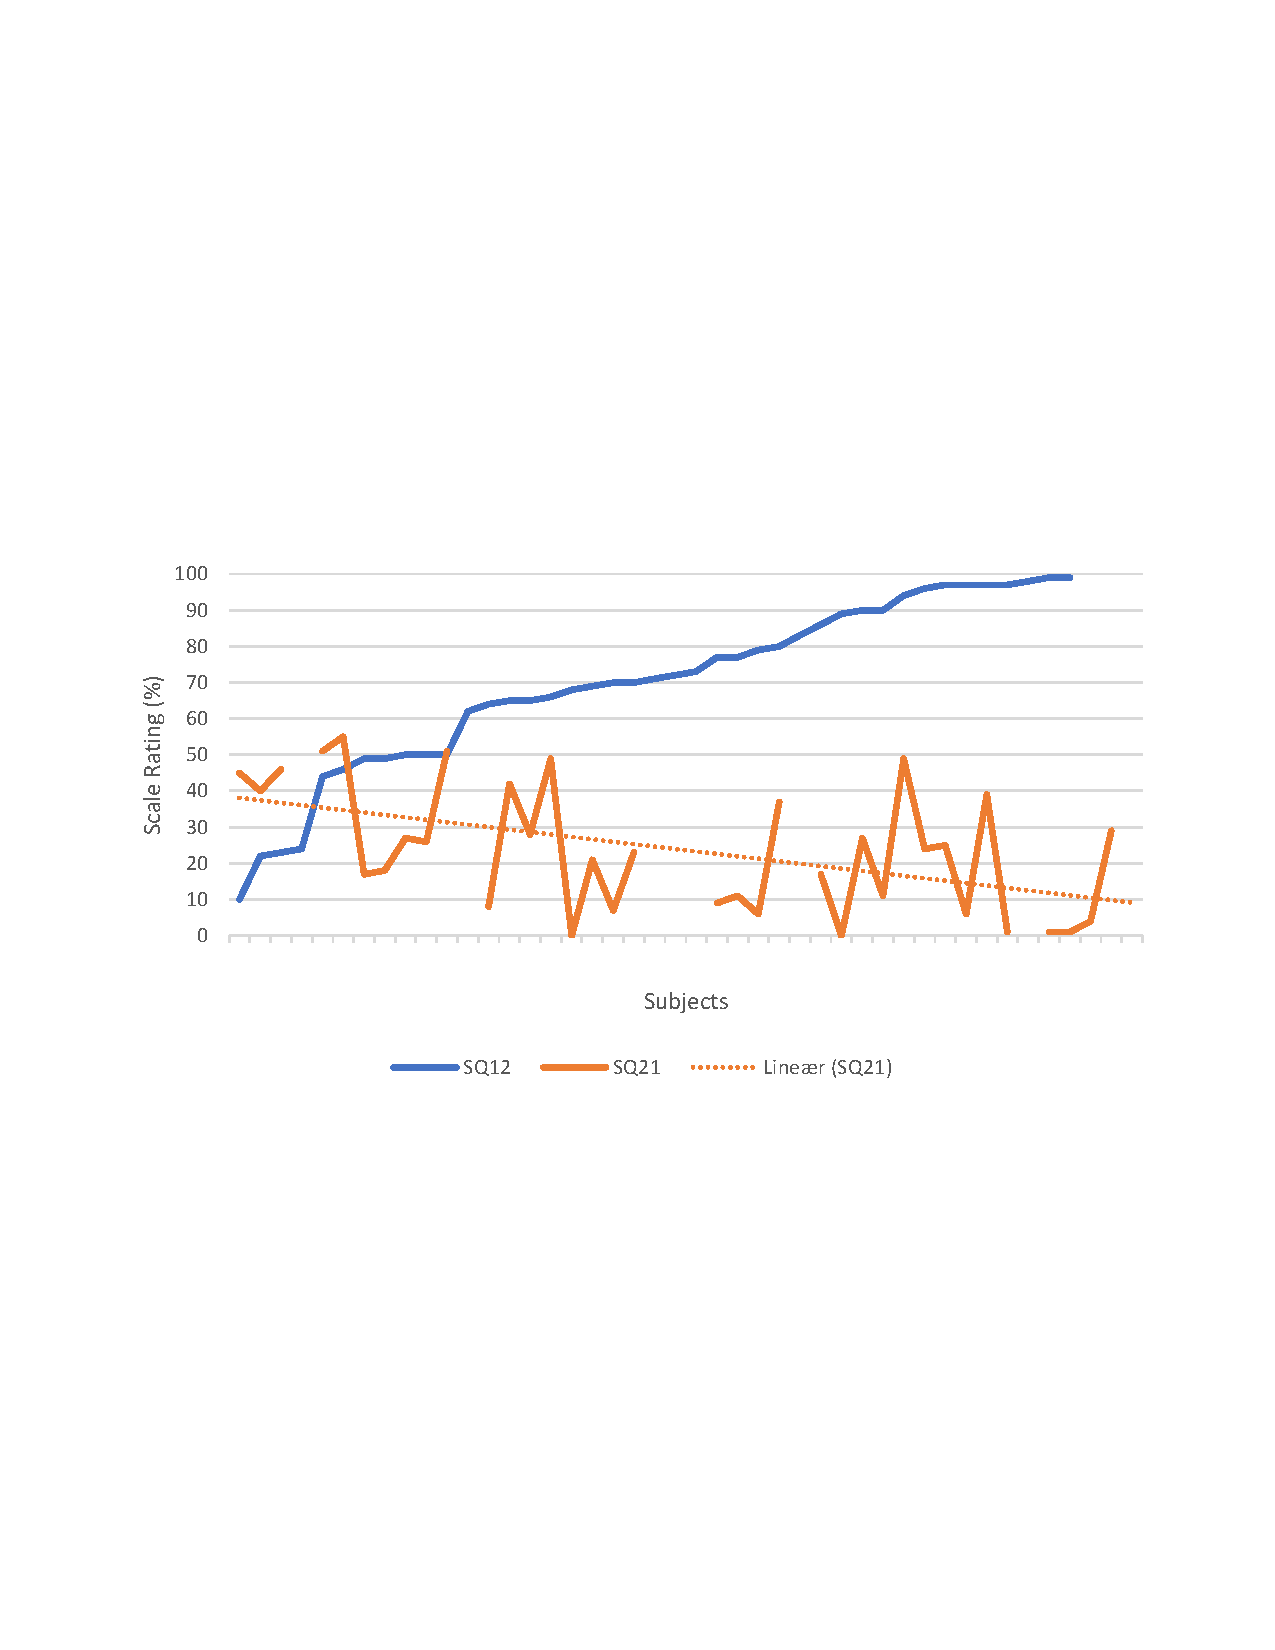
\includegraphics[width=\textwidth]{Figure/Korrelationsgrafer/SQ12+SQ21}
	\caption{Sammenhæng mellem hvad testpersonerne angiver (\%) på skalaen til SQ12: \textit{Jeg kan godt lide at blive betjent af robotten} og SQ21: \textit{Hvad synes du ellers om robotten?}. At den orange kurve ikke er kontinuerlig skyldes, at nogle testpersoner ikke har angivet en respons på skalaen.}
	\label{fig:SammenligningSQ12SQ21}
\end{figure}
\noindent
%
\autoref{fig:SammenligningSQ18SQ21} viser sammenhængen mellem SQ18 og SQ21. Her ses det, at det er en sammenhæng i testpersonernes ratings, da robotten anses som værende mindre anmasende, når robotten anses som værende mere spændende.
%
\begin{figure}[H]
	\centering
	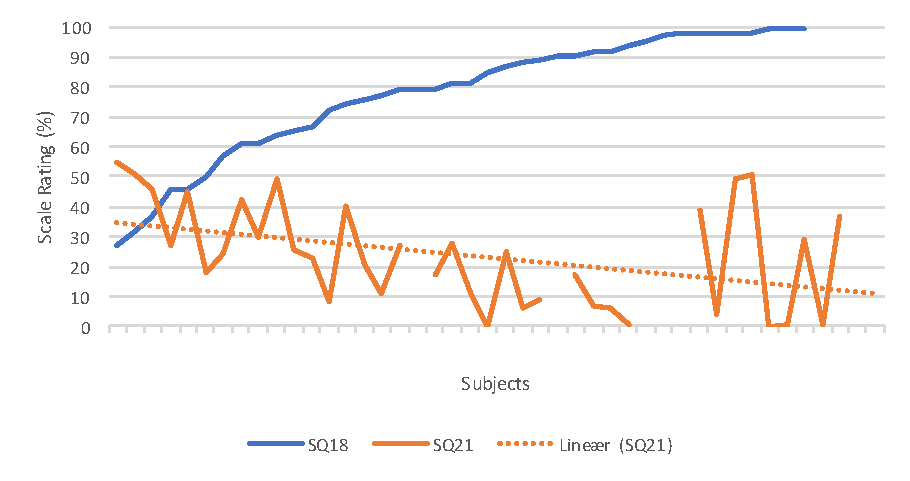
\includegraphics[width=\textwidth]{Figure/Korrelationsgrafer/SQ18+SQ21}
	\caption{Sammenhæng mellem hvad testpersonerne angiver (\%) på skalaen til SQ18: \textit{Hvad synes du om robotten} og SQ21: \textit{Hvad synes du ellers om robotten?}. At den orange kurve ikke er kontinuerlig skyldes, at nogle testpersoner ikke har angivet en respons på skalaen.}
	\label{fig:SammenligningSQ18SQ21}
\end{figure}
\noindent
%
På \autoref{fig:SammenligningSQ2SQ9} ses sammenhængen mellem SQ2 og SQ9. Figuren viser en tendens for, at ratings omkring hvorvidt robotten stod i vejen falder, når robotten opleves som mere imødekommende.
%
\begin{figure}[H]
	\centering
	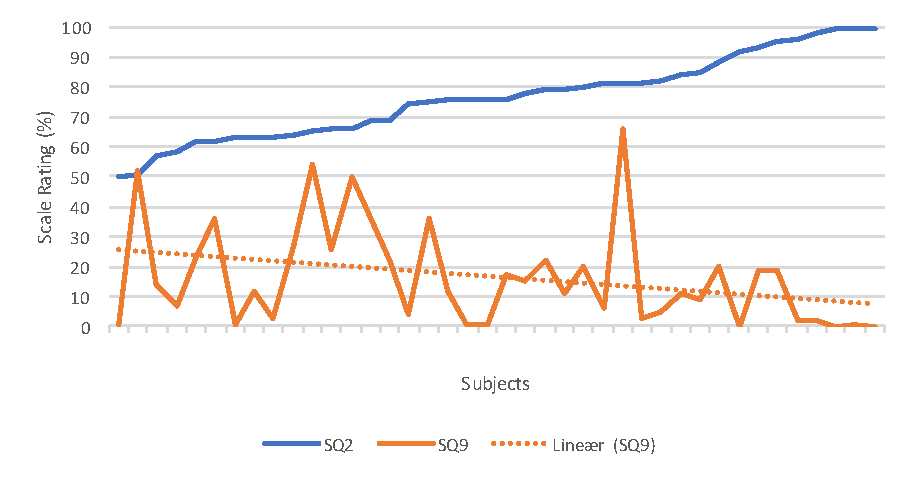
\includegraphics[width=\textwidth]{Figure/Korrelationsgrafer/SQ2+SQ9}
	\caption{Sammenhæng mellem hvad testpersonerne angiver (\%) på skalaen til SQ2: \textit{Hvordan oplevede du robotten?} og SQ9: \textit{Jeg synes, at robotten stod i vejen}. At den orange kurve ikke er kontinuerlig skyldes, at nogle testpersoner ikke har angivet en respons på skalaen.}
	\label{fig:SammenligningSQ2SQ9}
\end{figure}
\noindent
%
Selvom \autoref{fig:RHeight-Biplot} vise en negativ korrelation mellem SQ4 og SQ9, ses det på \autoref{fig:SammenligningSQ4SQ9}, at dette ikke nødvendigvis er tilfældet.
%
\begin{figure}[H]
	\centering
	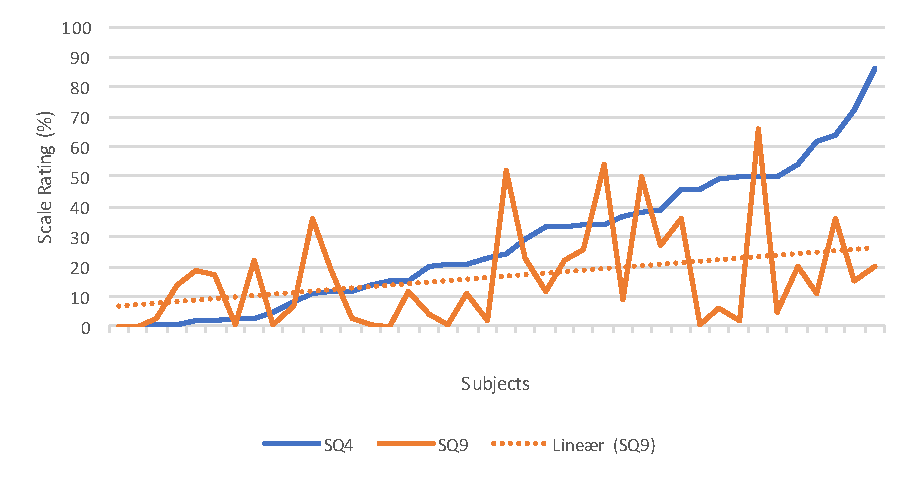
\includegraphics[width=\textwidth]{Figure/Korrelationsgrafer/SQ4+SQ9}
	\caption{Sammenhæng mellem hvad testpersonerne angiver (\%) på skalaen til SQ4: \textit{Hvordan oplevede du robottens bevægelser?} og SQ9: \textit{Jeg synes, at robotten stod i vejen}. At den orange kurve ikke er kontinuerlig skyldes, at nogle testpersoner ikke har angivet en respons på skalaen.}
	\label{fig:SammenligningSQ4SQ9}
\end{figure}
\noindent
%
\autoref{fig:SammenligningSQ16SQ19} ses sammenhængen mellem SQ16 og SQ19, hvor der ses en lille tendens af at testpersonerne synes robotten var mindre sød jo mere irriterende de synes den var. 
%
\begin{figure}[H]
	\centering
	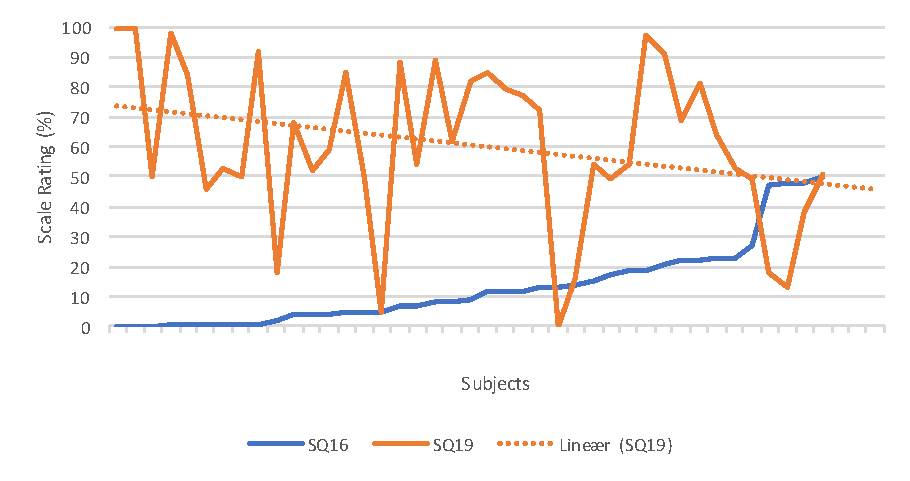
\includegraphics[width=\textwidth]{Figure/Korrelationsgrafer/SQ16+SQ19}
	\caption{Sammenhæng mellem hvad testpersonerne angiver (\%) på skalaen til SQ16 og SQ19, der begge har samme skala spørgsmål: \textit{Hvad synes du om robotten?} og forskellige labels.}
	\label{fig:SammenligningSQ16SQ19}
\end{figure}

\subsubsection{Korrelation relativt til afstand}
Når PCA analysen udføres relativt til afstand, tyder det, som beskrevet i \fullref{DatabehandlingRAfstand}, på, at en positiv korrelation mellem følgende parametre finder sted:
\begin{itemize}
	\item SQ1 og SQ12
	\item SQ7 og SQ17
	\item SQ10 og SQ22
	\item SQ8 og SQ21
\end{itemize}
%
Derudover ses der negativ korrelation mellem følgende parametre:
\begin{itemize}
	\item SQ2 og SQ9
	\item SQ14 og SQ16
	\item SQ10 og SQ13
	\item SQ13 og SQ22
	\item SQ5 og SQ8
	\item SQ5 og SQ21
	\item SQ19 og SQ20
\end{itemize}

Laves graferne for sammenhængen for SQ1 og SQ12 samt SQ7 og SQ17 ses der ikke nogen relevant sammenhæng, hvorfor disse kun er at finde i det elektroniske bilag, \fullref{ELEKTRONISK BILAG}.
På \autoref{fig:SammenligningSQ10SQ22} ses sammenhængen mellem SQ10 og SQ22. Det ses at der en lille tendens af, at testpersonerne synes robotten er mere sjov, når de samtidig føler sig mere tryg ved robotten.
%
\begin{figure}[H]
	\centering
	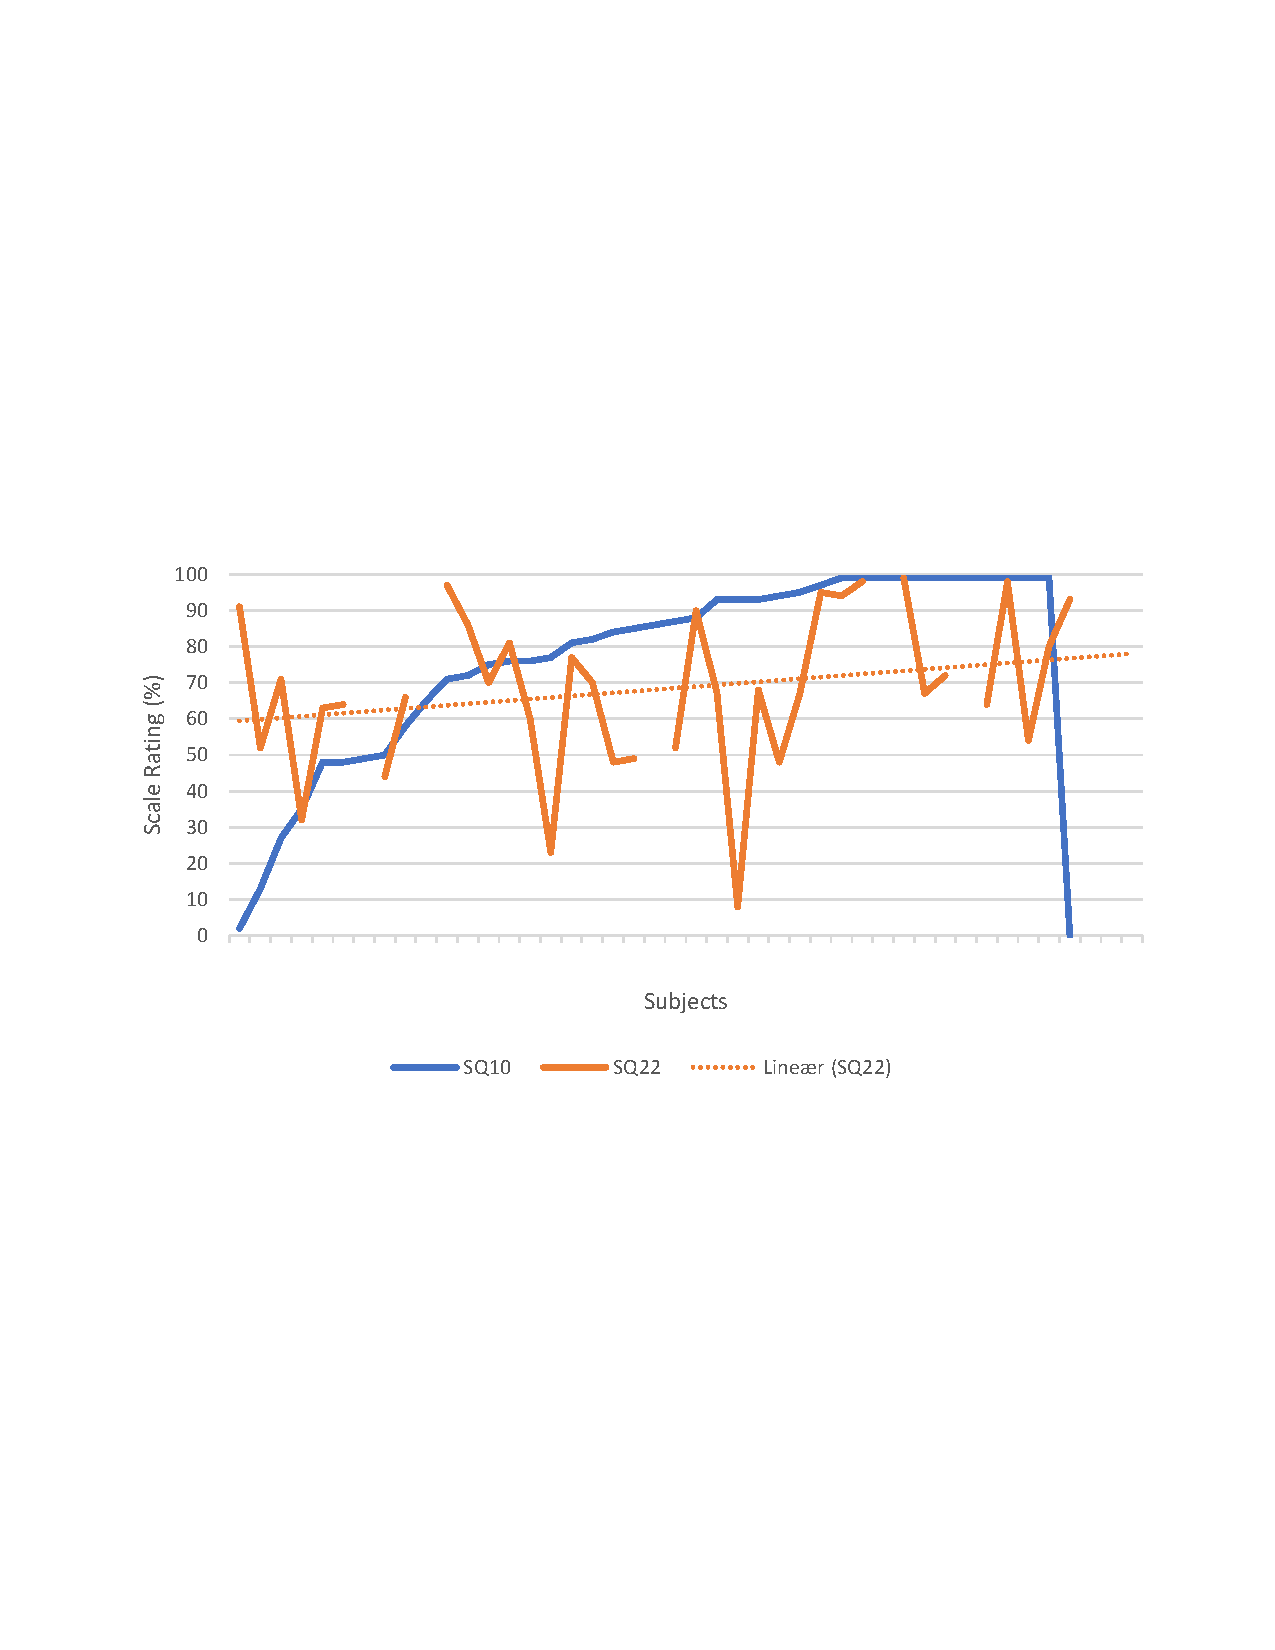
\includegraphics[width=\textwidth]{Figure/Korrelationsgrafer/SQ10+SQ22}
	\caption{Sammenhæng mellem hvad testpersonerne angiver (\%) på skalaen til SQ10: \textit{Jeg føler mig tryg ved robotten} og SQ22: \textit{Hvad synes du ellers om robotten?}. At den orange kurve ikke er kontinuerlig skyldes, at nogle testpersoner ikke har angivet en respons på skalaen.}
	\label{fig:SammenligningSQ10SQ22}
\end{figure}
\noindent
%
På \autoref{fig:SammenligningSQ8SQ21} vises sammenhængen mellem SQ8 og SQ21. Det forventes at tendenslinjen stiger i stedet for at falde, da en positiv korrelation mellem SQ8 og SQ21 er påvist på \autoref{fig:Distance-Biplot}. Dette er ikke nødvendigvis tilfældet, hvilket kan indikere at robotten findes mindre anmasende, når testpersonerne føler, at robotten kan hjælpe dem. 
%
\begin{figure}[H]
	\centering
	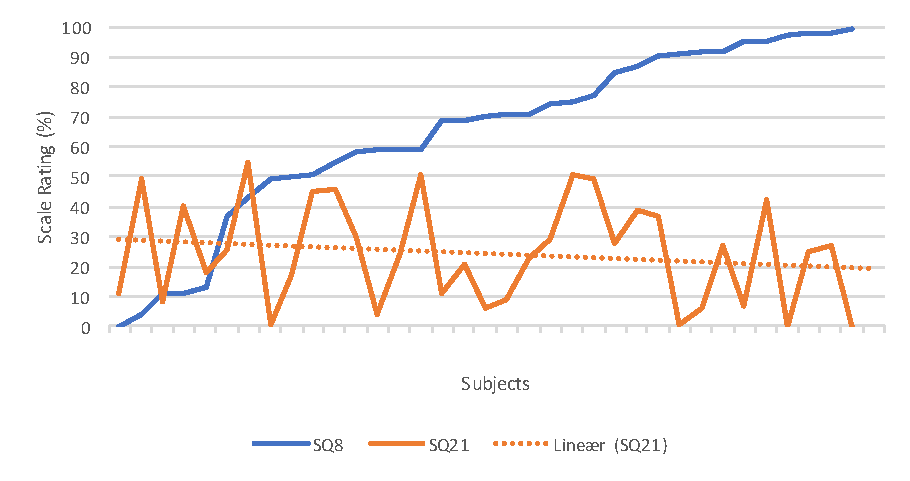
\includegraphics[width=\textwidth]{Figure/Korrelationsgrafer/SQ8+SQ21}
	\caption{Sammenhæng mellem hvad testpersonerne angiver (\%) på skalaen til SQ8: \textit{Jeg føler, at robotten kan hjælpe mig} og SQ21: \textit{Hvad synes du ellers om robotten?}. At den orange kurve ikke er kontinuerlig skyldes, at nogle testpersoner ikke har angivet en respons på skalaen.}
	\label{fig:SammenligningSQ8SQ21}
\end{figure}
\noindent
%
Undersøges den negative korrelation er sammenhængen mellem SQ2 og SQ9 allerede vist på \autoref{fig:SammenligningSQ2SQ9}. På \autoref{fig:SammenligningSQ14SQ16} vises sammenhængen for SQ14 og SQ16, hvor der ses en lille tendens for at robotten opleves som mindre sej, når den opleves som mere personlig.
%
\begin{figure}[H]
	\centering
	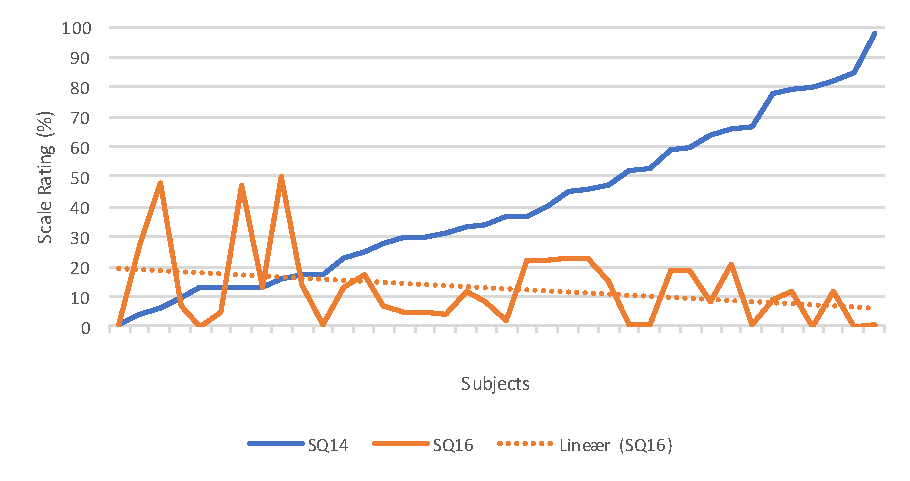
\includegraphics[width=\textwidth]{Figure/Korrelationsgrafer/SQ14+SQ16}
	\caption{Sammenhæng mellem hvad testpersonerne angiver (\%) på skalaen til SQ14: \textit{Hvor personlig oplevede du robottens hjælp?} og SQ16: \textit{Hvad synes du om robotten?}. At den orange kurve ikke er kontinuerlig skyldes, at nogle testpersoner ikke har angivet en respons på skalaen.}
	\label{fig:SammenligningSQ14SQ16}
\end{figure}
\noindent
%
Laves graferne for SQ10 og SQ13, SQ13 og SQ22 samt SQ19 og SQ20, vedlagt i \fullref{ELEKTRONISK BILAG}, ses det at graferne stiger samtidig. Dette er ikke forventet, da \autoref{fig:Distance-Biplot} viser en negativ korrelation ved disse parametre. Dog indikerer graferne at testpersonerne regnede med at blive fugt det sted de havde valgt, når de stolede på robotten og at robotten var sjov, når de troede de blev fulgt det rigtige sted hen. Ydermere indikerer graferne, at robotten blev perciperet som sej, når den også blev perciperet som sød.
Sammenlignes SQ5 og SQ8, jævnfør \autoref{fig:SammenligningSQ5SQ8}, er det svært at udlede, hvorvidt parametrene afhænger af hinanden eller følges ad ved tilfældighed. På trods af tidligere vist negativ korrelation relateret til afstand, virker det ikke til at testpersonerne har en ændret oplevelse af om robotten kan hjælpe dem, når robotten stopper tættere på eller længere væk. Det samme gør sig gældende, når SQ5 og SQ21 sammenlignes, hvilket kan ses på figuren i \fullref{ELEKTRONISK BILAG}. 

\begin{figure}[H]
	\centering
	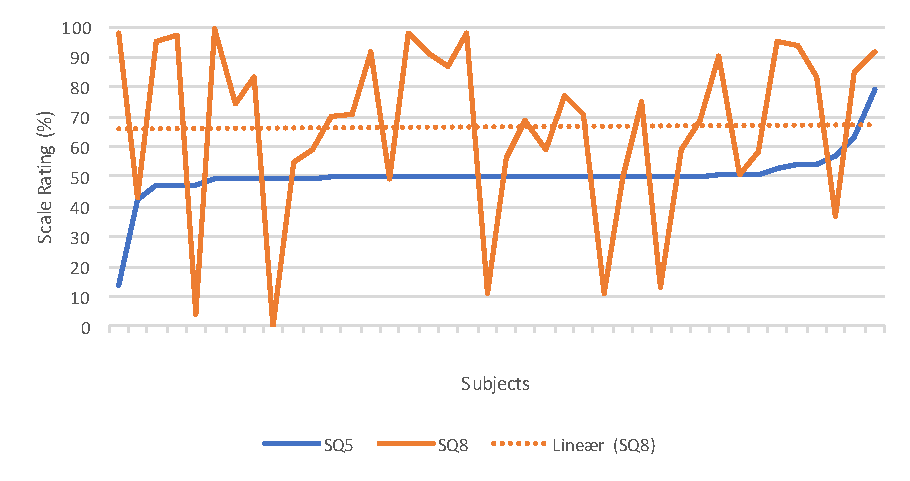
\includegraphics[width=\textwidth]{Figure/Korrelationsgrafer/SQ5+SQ8}
	\caption{Sammenhæng mellem hvad testpersonerne angiver (\%) på skalaen til SQ5: \textit{Jeg synes robotten stoppede...} og SQ8: \textit{Jeg føler, at robotten kan hjælpe mig}. At den orange kurve ikke er kontinuerlig skyldes, at nogle testpersoner ikke har angivet en respons på skalaen.}
	\label{fig:SammenligningSQ5SQ8}
\end{figure}
\noindent
%





\subsubsection{Korrelation relativt til indgangsvinkel}
Når PCA analysen udføres relativt til højde, tyder det, som beskrevet i \fullref{DatabehandlingRHeight}, på, at en positiv korrelation mellem følgende parametre finder sted:
\begin{itemize}
	\item SQ8 og SQ10
	\item SQ9 og SQ14
	\item SQ5 og SQ7
\end{itemize}
%
Derudover ses der negativ korrelation mellem følgende parametre:
\begin{itemize}
	\item SQ1 og SQ12
	\item SQ9 og SQ10
	\item SQ10 og SQ14
	\item SQ6 og SQ23
	\item SQ13 og S21
\end{itemize}